\chapter{Basics of Recursive Bayesian Estimation}

In following sections the problem of recursive Bayesian estimation (Bayesian filtering) is
stated and its analytical solution is derived. Later on, due to practical intractability of the
solution in its general form, a few methods that either simplify the problem or approximate the
solution are shown.

\section{Problem Statement}

Assume a dynamic system described by a hidden real-valued \emph{state vector} \(x\) which evolves at
discrete time steps according to a known function \(f_t\) (in this text called \emph{process model})
as described by \eqref{eq:DynSysFt}.
\begin{equation} \label{eq:DynSysFt}
	x_t = f_t(x_{t-1}, v_{t-1})
\end{equation}

Variable \(v_t\) in \eqref{eq:DynSysFt} denotes random \emph{process noise}, which may come from various
sources and is often inevitable. Sequence of \(v_t\) is assumed to be identically independently
distributed random variable sequence.

The state of the system is hidden and can only be observed though a real-valued \emph{observation vector}
\(y\) that relates to the state \(x\) as in \eqref{eq:DynSysHt}, but adds further \emph{observation
noise} \(w\).
\begin{equation} \label{eq:DynSysHt}
	y_t = h_t(x_t, w_t)
\end{equation}

In \eqref{eq:DynSysHt} \(h_t\) is known function called \emph{observation model} in this text and \(w_t\) is
identically independently distributed random variable sequence that denotes observation noise.

The goal of recursive\footnote{by the word recursive we mean that it is not needed to keep track of
the whole batch of previous observations in practical methods, only appropriate quantities from time
moments \(t-1\) and \(t\) are needed to estimate \(x_t\). However, this does not apply to the
derivation of the solution, where the notation of whole batch of observations \(y_{1:t}\) is used.}
Bayesian estimation is to give an estimate of the state \(x_t\) given the
observations \(y_{1:t}\) provided the knowledge of the functions \(f_t\) and \(h_t\).
More formally, the goal is to find the {\pdf} \(p(x_t | y_{1:t})\).
Theoretical solution to this problem is known and is presented in next section.

\section{Theoretical solution}

At first, we observe that {\pdf} \(p(x_t|x_{t-1})\) can be derived from the process model
\eqref{eq:DynSysFt} (given the distribution of \(v_k\)) and that \(p(y_t|x_t)\) can be derived from
the observation model \eqref{eq:DynSysHt} respectively. (given the distribution of \(w_k\))

Because recursive solution is requested, suppose that \(p(x_{t-1}|y_{1:t-1})\) and
\(p(x_0)\) are known\footnote{\(p(x_0)\) can be called initial {\pdf} of the state vector.} in
order to be able to make the transition \(t-1 \; \rightarrow \; t\).

In the first stage that can be called \emph{prediction}, \emph{prior} {\pdf}
\(p(x_t | y_{1:t-1})\) is calculated without knowledge of \(y_t\). We begin the derivation by
performing the reverse of the marginalization over \(x_{k-1}\).
\begin{equation*}
	p(x_t | y_{1:t-1}) = \int_{-\infty}^{\infty} p(x_t, x_{t-1} | y_{1:t-1}) \; \dx_{t-1}
\end{equation*}

Using chain rule for {\pdfs}, the element of integration can be split.
\begin{equation*}
	p(x_t | y_{1:t-1}) = \int_{-\infty}^{\infty} p(x_t | x_{t-1}, y_{1:t-1}) p(x_{t-1} | y_{1:t-1}) \; \dx_{t-1}
\end{equation*}

With an assumption that the modelled dynamic system \eqref{eq:DynSysFt} possesses \emph{Markov
Property}\footnote{an assumption of independence that states that system state in time \(t\) only
depends on system state in \(t-1\) (and is not directly affected by previous states).},
\(p(x_t | x_{t-1}, y_{1:t-1})\) equals \(p(x_t | x_{t-1})\).~\cite{AruMasGor:02}
This leaves us with the result \eqref{eq:PriorPdf}.
\begin{equation} \label{eq:PriorPdf}
	p(x_t | y_{1:t-1}) = \int_{-\infty}^{\infty} p(x_t | x_{t-1}) p(x_{t-1} | y_{1:t-1}) \; \dx_{t-1}
\end{equation}

As we can see, prior {\pdf} only depends on previously known functions and therefore can be
calculated.

We continue with the second stage that could be named \emph{update}, where new observation \(y_t\) is taken into
account and \emph{posterior} {\pdf} \(p(x_t | y_{1:t})\) is calculated. Bayes' theorem can be used
to derive posterior {\pdf} \eqref{eq:PosteriorPdfRaw}.
\begin{equation} \label{eq:PosteriorPdfRaw}
	p(x_t | y_{1:t}) = \frac{p(y_t | x_t, y_{1:t-1}) p(x_t | y_{1:t-1})}{p(y_t | y_{1:t-1})}
\end{equation}

According to the observation model \eqref{eq:DynSysHt} and assuming Markov property, \(y_t\) only
depends on \(x_t\). That is \(p(y_t | x_t, y_{1:t-1}) = p(y_t | x_t)\). Therefore posterior
{\pdf} can be further simplified into \eqref{eq:PosteriorPdf}.
\begin{equation} \label{eq:PosteriorPdf}
	p(x_t | y_{1:t}) = \frac{p(y_t | x_t) p(x_t | y_{1:t-1})}{p(y_t | y_{1:t-1})}
\end{equation}

While both {\pdfs} in the numerator of \eqref{eq:PosteriorPdf} are already known, \(p(y_t|y_{1:t-1})\)
found in the denominator can be calculated using the formula \eqref{eq:MargLikelihood}, where
marginalization over \(x_t\) is preformed. Quantity \eqref{eq:MargLikelihood} can also be interpreted as
\emph{marginal likelihood} (sometimes called \emph{evidence}) of observation.~\cite{Smi:10}
\begin{equation} \label{eq:MargLikelihood}
	p(y_t | y_{1:t-1}) = \int_{-\infty}^{\infty} p(y_t | x_t) p(x_t | y_{1:t-1}) \; \dx_{t}
\end{equation}

Computing \eqref{eq:MargLikelihood} isn't however strictly needed as it does not depend on \(x_t\) and
serves as a normalising constant in \eqref{eq:PosteriorPdf}. Depending on use-case the normalising
constant may not be needed at all or may be computed alternatively using the fact that \(p(x_t | y_{1:y})\)
integrates to \(1\).

We have shown that so called \emph{optimal Bayesian solution}\cite{AruMasGor:02} can be easily
analytically inferred using only \emph{chain rule for {\pdfs}}, \emph{marginalization} and
\emph{Bayes' theorem}. (equations \eqref{eq:PriorPdf}, \eqref{eq:PosteriorPdf} and
\eqref{eq:MargLikelihood} forming the main steps of the solution) On the other hand, using this
method directly in practice proves difficult because at least one parametric multidimensional
integration has to be performed (in \eqref{eq:PriorPdf}), which is (in its general form) hardly
tractable for greater than small state vector dimensions.

This is a motivation for various simplifications and approximations among which we have chosen
a Kalman filter described in the next section and a family of particle filters described later.

\section{Kalman Filter}

The Kalman filter\footnote{first presented by Rudolf Emil Kalman in 1960.} poses additional set of strong
assumptions on modelled dynamic system, but greatly
simplifies the optimal Bayesian solution \eqref{eq:PriorPdf}, \eqref{eq:PosteriorPdf} into a
sequence of algebraic operations with matrices. On the other hand, when these requirements can be
fulfilled, there is no better estimator in the Bayesian point of view because the Kalman filter computes
\(p(x_t | y_{1:t})\) \emph{exactly.}\footnote{not accounting for numeric errors that arise in
practical implementations.}

Assumptions additionally posed on system by the the Kalman filter are:
\begin{enumerate}
	\item \(f_t\) in the process model \eqref{eq:DynSysFt} is a linear function of \(x_t\) and
	\(v_t\).
	\item \(v_t \sim \mathcal{N}(0, Q_t)\) meaning that process noise \(v_t\) is normally
	distributed with zero mean\footnote{zero mean assumption is not strictly needed, it is however
	common in many implementations.} and with known covariance matrix \(Q_t\).
	\item \(h_t\) in the observation model \eqref{eq:DynSysHt} is a linear function of \(x_t\) and
	\(w_t\).
	\item \(w_t \sim \mathcal{N}(0, R_t)\) meaning that observation noise \(w_t\) is normally distributed
	with zero mean and with known covariance matrix \(R_t\).
	\item initial state {\pdf} is Gaussian.
\end{enumerate}

It can be proved that if the above assumptions hold, \(p(x_t|y_{1:t})\) is Gaussian for all
\(t > 0\).~\cite{Pet:81} Furthermore, given assumptions 1. and 2. the process model
\eqref{eq:DynSysFt} can be reformulated as \eqref{eq:LinSysAt}, where \(A_t\) is real-valued matrix
that represents \(f_t\).
Using the same idea and assumptions 3. and 4. the observation model \eqref{eq:DynSysHt} can be
expressed as \eqref{eq:LinSysCt}, \(C_t\) being real-valued matrix representing \(h_t\). Another
common requirement used below in the algorithm description is that \(v_t\) and \(w_t\) are
stochastically independent.
\begin{align}
	x_t &= A_t x_{t-1} + \hat{v}_{t-1} & A_t &\in \mathbb{R}^{n,n} \;\; n \in \mathbb{N} \label{eq:LinSysAt} \\
	y_t &= C_t x_t + \hat{w}_t & C_t &\in \mathbb{R}^{j,n} \;\; j \in \mathbb{N} \;\; j \leq n \label{eq:LinSysCt}
\end{align}

Note that we have marked the noises \(v_t\) and \(w_t\) as \(\hat{v}_t\) and \(\hat{w}_t\) when they
are transformed through \(A_t\), respectively \(C_t\) matrix. Let also \(\hat{Q}_t\) denote the
covariance matrix of \(\hat{v}_t\) and \(\hat{R}_t\) denote the covariance matrix of \(\hat{w}_t\)
in further text.

At this point we can describe the algorithm of the Kalman filter. As stated above, posterior {\pdf}
is Gaussian and thus can be parametrised by mean vector \(\mu\) and covariance matrix \(P\). Let us
denote posterior mean from previous iteration by \(\mu_{t-1|t-1}\) and associated covariance by
\(P_{t-1|t-1}\) as in \eqref{eq:KalmanPreAPost}.
\begin{equation} \label{eq:KalmanPreAPost}
	p(x_{t-1} | y_{1:t-1}) = \mathcal{N}(\mu_{t-1|t-1}, P_{t-1|t-1})
\end{equation}

Prior {\pdf} \eqref{eq:KalmanAPrior} can then be calculated as follows:~\cite{AruMasGor:02}
\begin{align}
	p(x_t | y_{1:t-1}) &= \mathcal{N}(\mu_{t|t-1}, P_{t|t-1}) \label{eq:KalmanAPrior} \\
	\mu_{t|t-1} &= A_t \mu_{t-1|t-1} \notag \\
	P_{t|t-1} &= A_t P_{t-1|t-1} A_t^T + \hat{Q}_{t-1} \notag
\end{align}

Before introducing posterior {\pdf} it is useful to establish another Gaussian {\pdf}
\eqref{eq:KalmanEvidence} that is not necessarily needed, but is useful because it represents
marginal likelihood \eqref{eq:MargLikelihood}. % TODO: citation for this!
\begin{align}
	p(y_t|y_{1:t-1}) &= \mathcal{N}(\nu_{t|t-1}, S_{t|t-1}) \label{eq:KalmanEvidence} \\
	\nu_{t|t-1} &= C_t \mu_{t|t-1} \notag \\
	S_{t|t-1} &= C_t P_{t|t-1} C_t^T + \hat{R}_t \notag
\end{align}

The update phase of the Kalman filter can be performed by computing so-called \emph{Kalman gain} matrix
\eqref{eq:KalmanGain}, posterior {\pdf} \eqref{eq:KalmanAPost} is then derived from prior one
using the Kalman gain \(K_t\) and observation \(y_t\).~\cite{AruMasGor:02}
\begin{align}
	K_t &= P_{t|t-1} C_t^T S_{t|t-1}^{-1} \label{eq:KalmanGain} \\[\parskip]
	p(x_t|y_{1:t}) &= \mathcal{N}(\mu_{t|t}, P_{t|t}) \label{eq:KalmanAPost} \\
	\mu_{t|t} &= \mu_{t|t-1} + K_t(y_t - \nu_{t|t-1}) \notag \\
	P_{t|t} &= P_{t|t-1} - K_t C_t P_{t|t-1} \notag
\end{align}

In all formulas above \(A^T\) denotes a transpose of matrix \(A\) and \(A^{-1}\) denotes inverse
matrix to \(A\). As can be seen, formulas \eqref{eq:PriorPdf} and \eqref{eq:PosteriorPdf} have
been reduced to tractable algebraic operations, computing inverse matrix\footnote{it can be shown
that \(S_{t|t-1}\) is positive definite given that \(C_t\) is full-ranked,
therefore the inverse in \eqref{eq:KalmanGain} exists.} being the most costly one.

\begin{figure}[h]
	\centering
	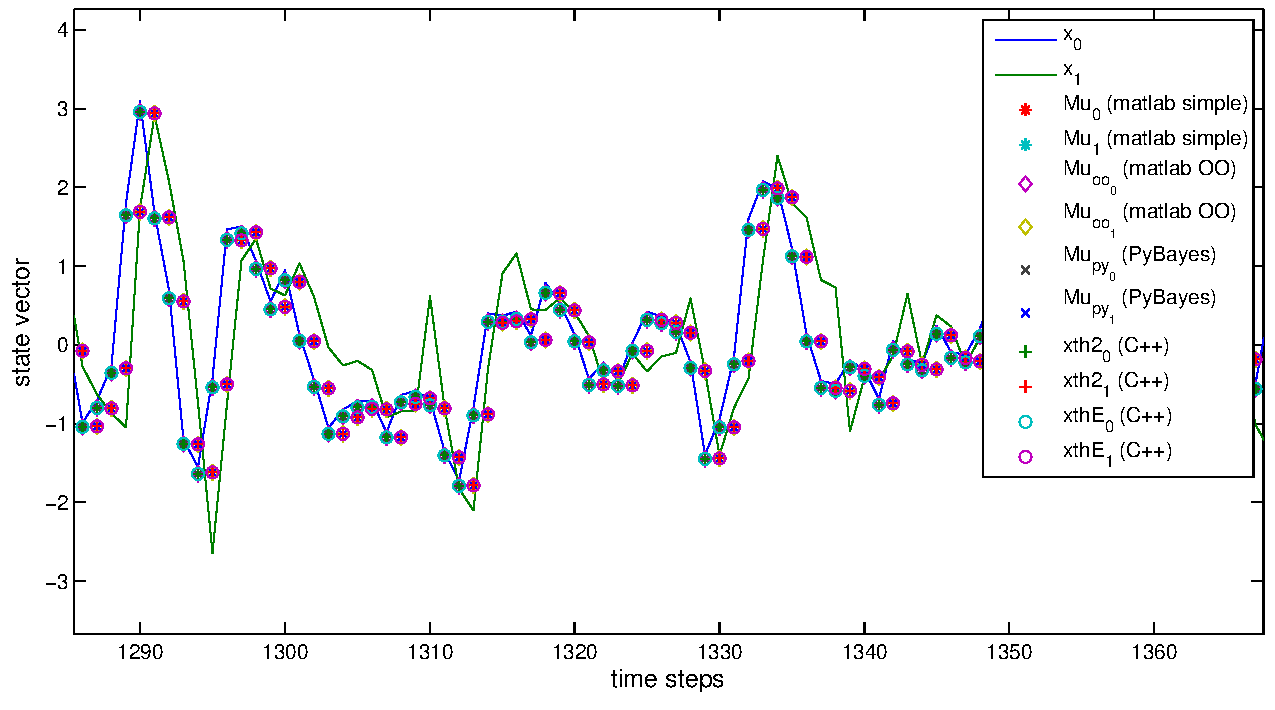
\includegraphics[width=\textwidth,keepaspectratio=true]{KF.pdf}
	\caption[Example run of the Kalman filter]{Example run of the Kalman filter. Lines are actual
	(hidden) state, dots estimation means of various implementations (all yielding the same values).}
	\label{fig:KF}
\end{figure}

It should be further noted that the Kalman filter and described algorithm can be easily enhanced to
additionally cope with an \emph{intervention} (or control) vector applied to the system, making it
suitable for the theory of decision-making. Numerous generalisations of the Kalman filter exist, for
example an \emph{extended Kalman filter} that relaxes the requirement of the linear system by locally
approximating a non-linear system with Taylor series. These are out of scope of this
text, but provide areas for subsequent consideration.

On the other hand, the assumption of Gaussian posterior {\pdf} cannot be easily overcome and for
systems that show out non-Gaussian distributions of the state vector another approach have to be
taken.~\cite{AruMasGor:02} One such approach can be a Monte Carlo-based \emph{particle filter}
presented in the next section.

\section{Particle Filter} \label{sec:ParticleFilter}

Particle filters represent approximate solution of the problem of the recursive Bayesian estimation,
thus can be considered \emph{suboptimal} methods. The underlying algorithm described below is most
commonly named \emph{sequential importance sampling (SIS)}. The biggest advantage of the particle filtering
is that requirements posed on the modelled system are much weaker than those assumed by optimal methods
such as the Kalman filter. Simple form of the particle filter presented in this section (that assumes that
modelled system has Markov property) requires only the knowledge of {\pdf} \(p(x_t|x_{t-1})\)
representing the process model and the knowledge of \(p(y_t|x_t)\) representing the observation
model.\footnote{both {\pdfs} are generally time-varying and their knowledge for all \(t\) is needed,
but their representation (parametrised by conditioning variable) is frequently constant in time in
practical applications.}

The sequential importance sampling approximates posterior density by a weighted empirical
{\pdf} \eqref{eq:PFAPost}.
\begin{align}
	p(x_t | y_{1:t}) \approx \sum_{i=1}^N \omega_t^{(i)} \delta(x_t - x_t^{(i)}) \label{eq:PFAPost} \\
	\forall i \in \mathbb{N} \;\; i \leq N: \omega_i \geq 0 \quad\quad \sum_{i=1}^N \omega_i = 1 \notag
\end{align}

In \eqref{eq:PFAPost} \(x_t^{(i)}\) denotes value of i-th \emph{particle}: possible state of the
system at time \(t\);
\(\omega_t^{(i)}\) signifies weight of i-th particle at time \(t\): scalar value proportional to
expected probability of the system being in state in small neighbourhood of \(x_t^{(i)}\);
\(N\) denotes total number of particles\footnote{\(N\) is assumed to be
arbitrary but fixed positive integer for our uses. Variants of the particle filter exist that use
adaptive number of particles, these are not discussed here.}, a significant tunable parameter
of the filter.

As the initial step of the described particle filter, \(N\) random particles are sampled
from the initial {\pdf}
\(p(x_0)\). Let \(i \in \mathbb{N} \;\; i \leq N\), transition \(t-1 \; \rightarrow \; t\) can be
performed as follows:
\begin{enumerate}
	\item for each \(i\) compute \(x_t^{(i)}\) by random sampling from conditional {\pdf}
		\(p(x_t|x_{t-1})\) where \(x_{t-1}^{(i)}\) substitutes \(x_{t-1}\) in condition. This step
		can be interpreted as a simulation of possible system state developments.
	\item for each \(i\) compute weight \(\omega_t^{(i)}\) using \eqref{eq:PFWeightUpdate}
		by taking observation \(y_t\) into account. \(x_t\) is substituted by \(x_t^{(i)}\) in
		condition in \eqref{eq:PFWeightUpdate}. Simulated system states are confronted with reality
		through observation.
		\begin{equation} \label{eq:PFWeightUpdate}
			\omega_t^{(i)} = p(y_t | x_t) \omega_{t-1}^{(i)}
		\end{equation}
	\item normalise weights according to \eqref{eq:PFWeightNormalise} so that approximation of
		posterior {\pdf} integrates to one.
		\begin{equation} \label{eq:PFWeightNormalise}
			\omega_t^{(i)} = \frac{\omega_t^{(i)}}{\sum_{j=1}^N \omega_t^{(j)}}
		\end{equation}
\end{enumerate}

Relative computational ease of described algorithm comes with
cost: first, the particle filter is in principle non-deterministic because of the random sampling in
step~1, in other words, the particle filter is essentially a Monte Carlo method; second, appropriate
number of particles \(N\) has to be chosen --- too small \(N\) can lead to significant approximation
error while inadequately large \(N\) can make the particle filter infeasibly time-consuming. It can be
proved that the particle filter converges to true posterior density as \(N\) approaches
infinity and certain other assumptions hold~\cite{CriDou:02}, therefore the number of particles
should be chosen as a~balance of accuracy and speed.

Only two operations with {\pdfs} were needed: sampling from \(p(x_t|x_{t-1})\) and evaluating
\(p(y_t | x_t)\) in known point. Sometimes sampling from \(p(x_t|x_{t-1})\) is not
feasible\footnote{but can be replaced by evaluation in known point.} and/or better results are
expected by taking an observation \(y_t\) into account during sampling (step~1). This can be
achieved by introducing so-called \emph{proposal density} (sometimes \emph{importance density})
\(q(x_t|x_{t-1}, y_t)\). Sampling in step~1 then uses \(q(x_t|x_{t-1}, y_t)\) instead, where \(x_{t-1}\) in
condition is substituted by \(x_{t-1}^{(i)}\). Weight computation in step~2 have to be replaced with
\eqref{eq:PFWeightUpdateProp} that compensates different sampling distribution (every occurrence of
\(x_t\), \(x_{t-1}\) in the mentioned formula has to be substituted by \(x_t^{(i)}\) and \(x_{t-1}^{(i)}\)
respectively). See \cite{AruMasGor:02} for a derivation of these formulas and for a discussion about
choosing adequate proposal density.
\begin{equation} \label{eq:PFWeightUpdateProp}
	\omega_t^{(i)} = \frac{p(y_t|x_t)p(x_t|x_{t-1})}{q(x_t|x_{t-1}, y_t)} \omega_{t-1}^{(i)}
\end{equation}

Particle filters also suffer from a phenomenon known as \emph{sample impoverishment} or
\emph{degeneracy problem}: after a few iterations all but one particles' weight falls close to
zero.\footnote{it has been shown that variance of particle weights continually raises as algorithm
progresses.~\cite{AruMasGor:02}}
One technique to diminish this is based on careful choice of proposal density (as explained in
\cite{AruMasGor:02}), a second one is to add additional \emph{resample} step to the above
algorithm:
\begin{enumerate}[resume] % so that enumeration starts with number 4
	\item for each \(i\) resample \(x_t^{(i)}\) from approximate posterior {\pdf}
		\(\sum_{i=1}^N \omega_t^{(i)} \delta(x_t - x_t^{(i)})\) and reset all weights to \(\frac{1}{N}\).
		Given that sampling is truly random and independent this means that each particle is in
		average copied \(n_i\) times, where \(n_i\) is roughly proportional to particle weight:
		\(n_i \approx \omega_t^{(i)} N\). Statistics of posterior {\pdf} are therefore (roughly and
		on average) maintained while low-weight particles are eliminated.
\end{enumerate}
Step~4 therefore facilitates avoidance of particles with negligible weight by replacing them with more weighted
ones. Such enhanced algorithm is known as \emph{sequential importance resampling (SIR)}.

Because particle resampling is computationally expensive operation, a technique can be used where
resampling is skipped in some iterations, based on the following idea:
a measurement of degeneracy can be obtained by computing an
approximate of \emph{effective sample size} \(N_{\text{eff}}\) at given time \(t\) using
\eqref{eq:PFNeff}.~\cite{AruMasGor:02}
\begin{equation} \label{eq:PFNeff}
	N_{\text{eff}} \approx \left( \sum_{i=1}^N \left( \omega_t^{(i)} \right)^2 \right)^{-1}
\end{equation}
Very small \(N_{\text{eff}}\) compared to \(N\) signifies a substantial loss of ``active'' particles,
which is certainly undesirable as it hurts accuracy while leaving computational demands unchanged.
Step~4 is then performed only when \(N_{\text{eff}}\) falls below certain threshold.

Recursive Bayesian estimation using SIR methods can be applied to a wide range of dynamic systems
(even to those where more specialised methods fail) and can be tuned with number of particles \(N\) and
proposal density \(q\). On the other hand a method specially designed for a given system easily
outperforms general particle filter in terms of speed and accuracy.

\section{Marginalized Particle Filter}

Main sources of this section are \cite{SchGusNor:05} and \cite{SchKarGus:06}.

The marginalized particle filter (sometimes \emph{Rao-Blackwellized particle filter}) is an
extension to the particle filter that more accurately approximates the optimal Bayesian solution
provided that the {\pdf} representing the process model \(p(x_t|x_{t-1})\) can be obtained in
a special form. Suppose that the state vector can be divided into two parts \(a_t\) and \(b_t\)
\eqref{eq:MPFStateVec} and that the process model {\pdf} can be expressed as a product of two
{\pdfs} \eqref{eq:MPFProcessMod}, where \(p(a_t|a_{t-1} b_t)\) is analytically tractable (in general).
We present a simple variant of the marginalized particle filter where, given \(b_t\), process and
observation model of the \(a_t\) part are linear with normally-distributed noise. The Kalman filter
can be used to estimate \(a_t\) part of the state vector in this case.
\begin{align}
	x_t &= (a_t, b_t) \label{eq:MPFStateVec} \\
	p(x_t|x_{t-1}) &= p(a_t, b_t|a_{t-1}, b_{t-1}) = p(a_t|a_{t-1}, b_t) p(b_t | b_{t-1}) \label{eq:MPFProcessMod}
\end{align}

The posterior {\pdf} \eqref{eq:MPFPosterior} can be represented as a product of a weighted empirical
distribution and a normal distribution. Each (i-th) particle is thus associated with its Kalman filter
(representing \(a_t^{(i)}\) part) and \(b_t^{(i)}\) quantity.
\begin{equation} \label{eq:MPFPosterior}
	p(a_t, b_t | y_t) = \sum_{i=1}^N \omega_i p(a_t|y_{1:t},b_{1:t}^{(i)}) \; \delta(b_t - b_t^{(i)})
\end{equation}

In \eqref{eq:MPFPosterior} \(N\) denotes the total number of particles, \(\omega_i\) denotes weight
of i-th particle, \(p(a_t|y_{1:t},b_{1:t}^{(i)})\) is posterior {\pdf} of i-th Kalman
filter and \(b_t^{(i)}\) is a value of the \(b_t\) part of i-th particle.

The algorithm of the described variant of the marginalized particle filter follows, note the
similarities with the ordinary particle filter: at first, generate \(N\) \(b_t\) random samples from
the initial distribution \(p(b_0)\). Then the following procedure can be repeated for each measurement
\(y_t\):
\begin{enumerate}
	\item for each \(i\) compute \(b_t^{(i)}\) by random sampling from conditional {\pdf}
		\(p(b_t|b_{t-1})\) where \(b_{t-1}^{(i)}\) substitutes \(b_{t-1}\) in condition.
	\item for each \(i\) compute the posterior {\pdf} \(p(a_t|y_{1:t},b_{1:t}^{(i)})\) of the i-th
		Kalman filter using \(y_t\) and \(b_t^{(i)}\).
	\item for each \(i\) update weight \(\omega_i\) using the formula \eqref{eq:MPFWeightUpdate} where
		marginal likelihood of the i-th Kalman filter \eqref{eq:KalmanEvidence} is used.
		\begin{equation} \label{eq:MPFWeightUpdate}
			\omega_i = p(y_t|y_{1:t},b_{1:t}^{(i)}) \; \omega_i
		\end{equation}
	\item normalise weights (as described in the previous section).
	\item resample particles (as described in the previous section).
\end{enumerate}

It has been demonstrated in various publications that the marginalised particle filter outperforms
the ordinary particle filter in both better accuracy and lower computational demands. Where
applicable, it therefore forms an excellent alternative to traditional particle filtering.
